\section{Classification}
\label{classification}
For our classification, we have worked with Logistic Regression, Decision Tree, K-nearest neighbours and Artificial Neural Network. All these methods have been applied, where we look at all the attributes of our dataset, where we only look at the attributes with the most importance according to our forward selection section \ref{ForwardSelection}, where we have standardized the data according to find principal components looking at all the principal components, and where we only look at the two most important principal components. Meaning we have given our data as four different types of input for these methods.

\subsection{Logistic Regression}

We have applied logistic regression to our data. For logistic regression, we calculate a value for each data object. This value can be used to estimate the likelihood of the object to be CHD positive.

\begin{figure}
	\begin{subfigure}[b]{0.5\textwidth}
	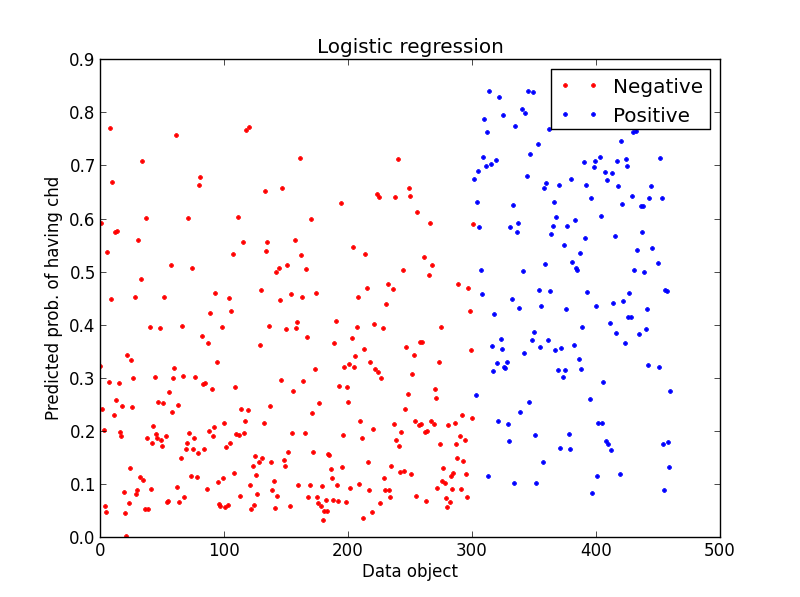
\includegraphics[scale=0.4]{pictures/logisticregressionX.png}
	\caption{Looking at all attributes.}
	\label{logicalRegressionResultX}
	\end{subfigure}
	\begin{subfigure}[b]{0.5\textwidth}
	\includegraphics[scale=0.4]{pictures/logisticregressionXad.png}	
	\caption{Looking at attributes selected by forward selection.}
	\label{logicalRegressionResultXad}
	\end{subfigure}

	\begin{subfigure}[b]{0.5\textwidth}
	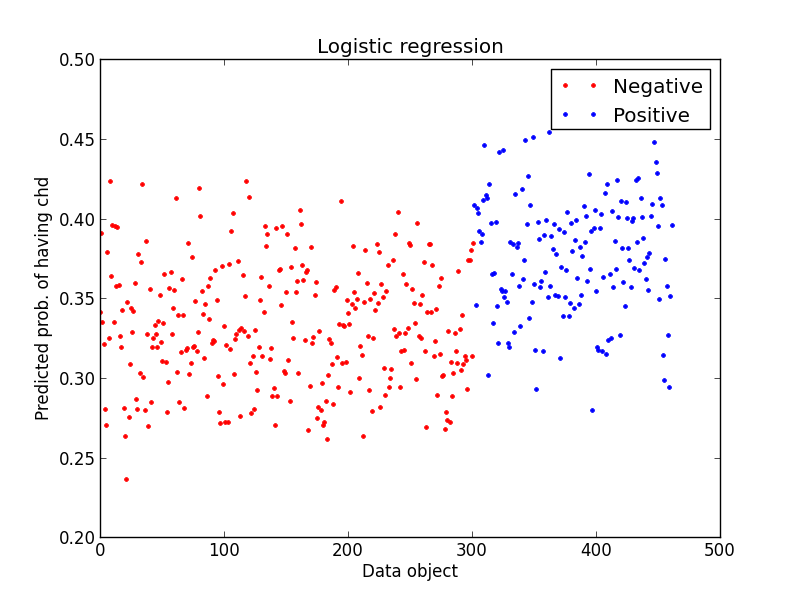
\includegraphics[scale=0.4]{pictures/logisticregressionXPC.png}
	\caption{Looking at all principal components.}
	\label{logicalRegressionResultXPA}
	\end{subfigure}
	\begin{subfigure}[b]{0.5\textwidth}
	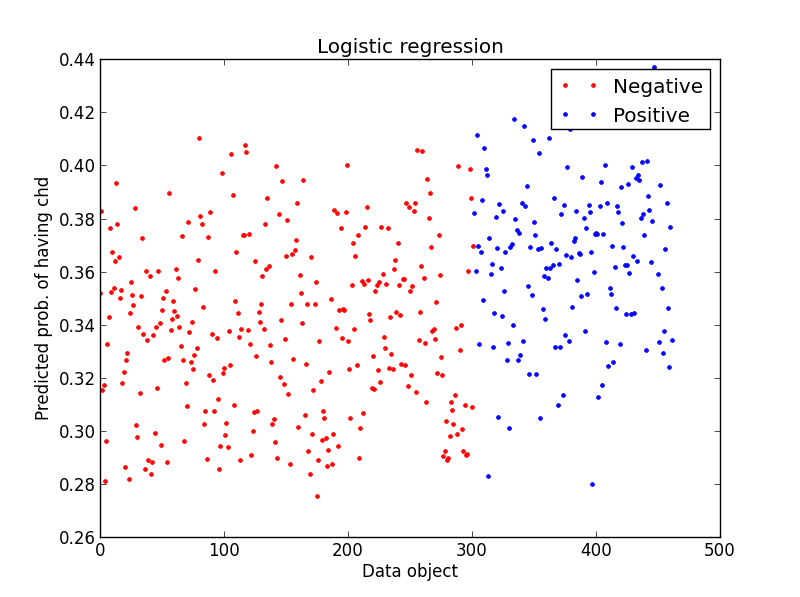
\includegraphics[scale=0.4]{pictures/logisticregressionX2PC.png}
	\caption{Looking at two most important principal components.}
	\label{logicalRegressionResultX2PA}
	\end{subfigure}
\caption{This figure shows results of performing logical regression for different input.}
\label{logicalRegressionResults}
\end{figure}

Se Figure \ref{logicalRegressionResults} to see output for our different input, when running Logistic Regression. Looking at Figure \ref{logicalRegressionResultX}, we see our results, when we have not alternated with the data, and likewise we see at Figure \ref{logicalRegressionResultXad}, our results for when, we have removed the attributes with less influence, meaning for this case we only look at the attributes: Age, Alcohol, Type-A, Family history, Low density lipoprotein cholesterol (LDL). For see especially from these to output of results that there is a tendency for subjects actually having the disease to have a higher probability of having the disease, even though we still see subjects having the disease with low predicted probability and likewise subjects not having the disease having a high predicted probability.

Looking at Figures \ref{logicalRegressionResultXPA} and \ref{logicalRegressionResultX2PA}, where we use principal components to give a logical regression of the data, also see a tendency of people actually having the disease, also have a higher predicted probability of having the disease. However we see that the interval of predicted probabilities are much less. Actually we see from these two graphs that all subjects have a predicted probability of less than 50\%.

A naive way of classifying subjects from these results, is classifying subjects with a predicted probability of more than 50\% as CHD-positive and vice versa the rest as being CHD-negative. This way we can go through all the subjects of the sets, and see how big a percentage are classified correct or wrong. This gives us the misclassification rate. These can be seen in Figure \ref{logicalRegressionErrorRate}

\begin{table}
\begin{longtable}{lc} \hline
Result from: & Mis-classification rate \\ \hline
Figure \ref{logicalRegressionResultX} & 26,6\% \\ 
Figure \ref{logicalRegressionResultXad} & 25,8\% \\ 
Figure \ref{logicalRegressionResultXPA} & 34,6\% \\ 
Figure \ref{logicalRegressionResultX2PA} & 34,6\% \\ \hline
\end{longtable}
\caption{Mis-classification rate for the logistic regressions.}
\label{logicalRegressionErrorRate}
\end{table}

We see that we actually get the smallest misclassification rate, when we look at the results from when we do not use principal component analysis, but we also see that in this case, we can use the results from our forward selection to decrease the misclassification result. For comparing these misclassification rates, we should compare to just classifying all objects to be negative. For this we get a misclassification rate of $\frac{160}{462}=34,6\%$, as we have 160 positive samples from a total of 462 samples. We see that this misclassification rate corresponds to the results described in Figures \ref{logicalRegressionResultXPA} and \ref{logicalRegressionResultX2PA}. This makes sense, since the predicted probability of all subjects in these cases are below 50\%.

\input{decisionTree}

\subsection{K-nearest neighbours}

The data set has been exposed to classification by looking at the k nearest neighbours.

\begin{figure}
	\begin{subfigure}[b]{0.5\textwidth}
	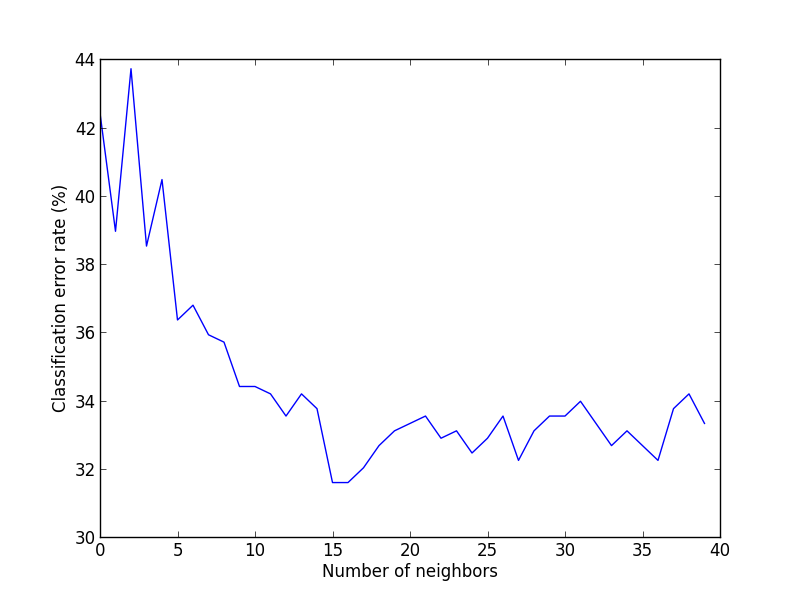
\includegraphics[scale=0.4]{pictures/knnX.png}
	\caption{Looking at all attributes.}
	\label{logicalRegressionResultX}
	\end{subfigure}
	\begin{subfigure}[b]{0.5\textwidth}
	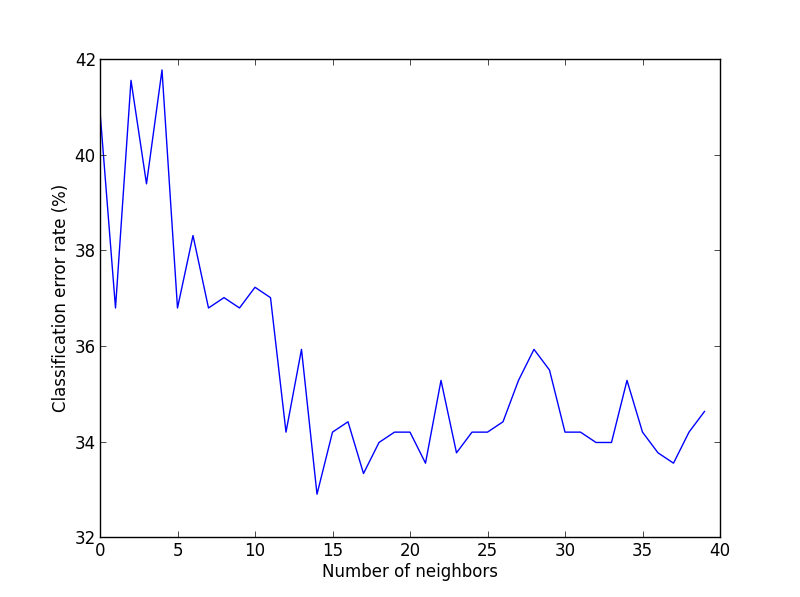
\includegraphics[scale=0.4]{pictures/knnXAD.png}	
	\caption{Looking at attributes selected by forward selection.}
	\label{logicalRegressionResultXad}
	\end{subfigure}

	\begin{subfigure}[b]{0.5\textwidth}
	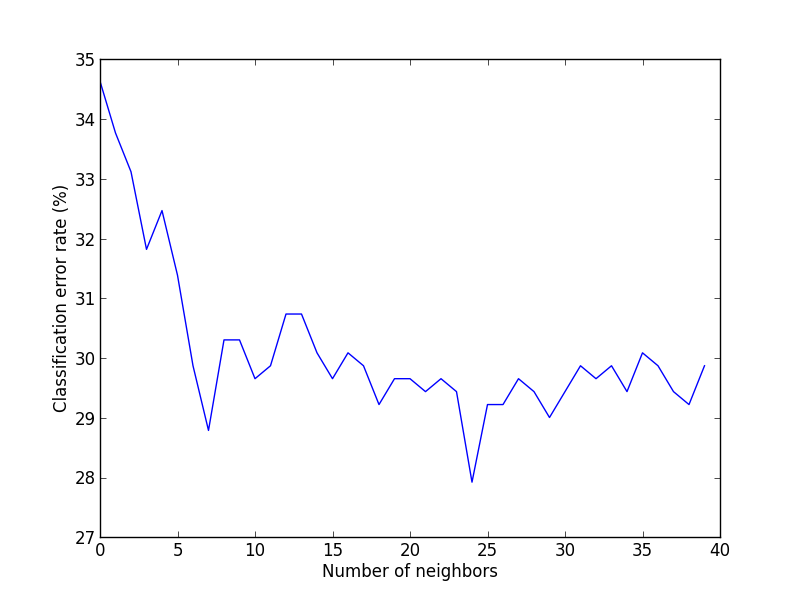
\includegraphics[scale=0.4]{pictures/knnPC.png}
	\caption{Looking at all principal components.}
	\label{logicalRegressionResultXPA}
	\end{subfigure}
	\begin{subfigure}[b]{0.5\textwidth}
	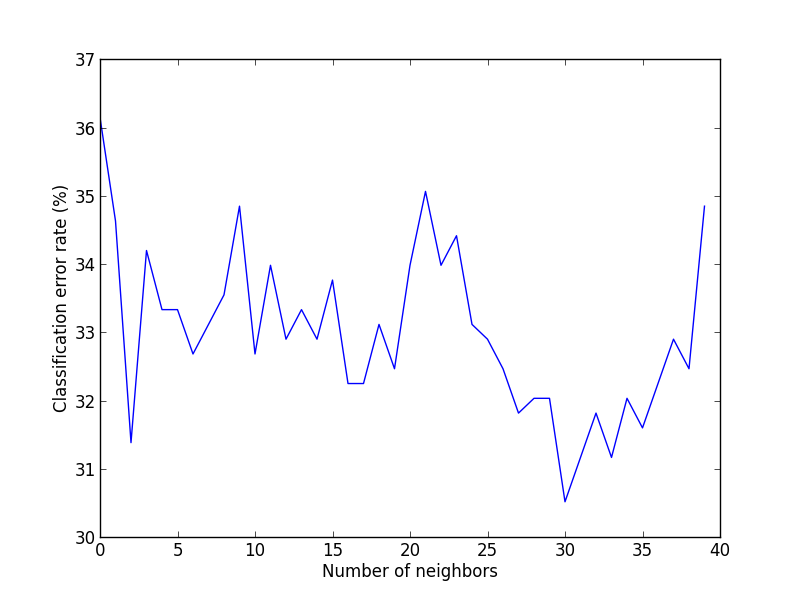
\includegraphics[scale=0.4]{pictures/knn2PC.png}
	\caption{Looking at two most important principal components.}
	\label{logicalRegressionResultX2PA}
	\end{subfigure}
\caption{This figure shows results of performing logical regression for different input.}
\label{logicalRegressionResults}
\end{figure}


\begin{figure}
	\begin{subfigure}[b]{0.5\textwidth}
	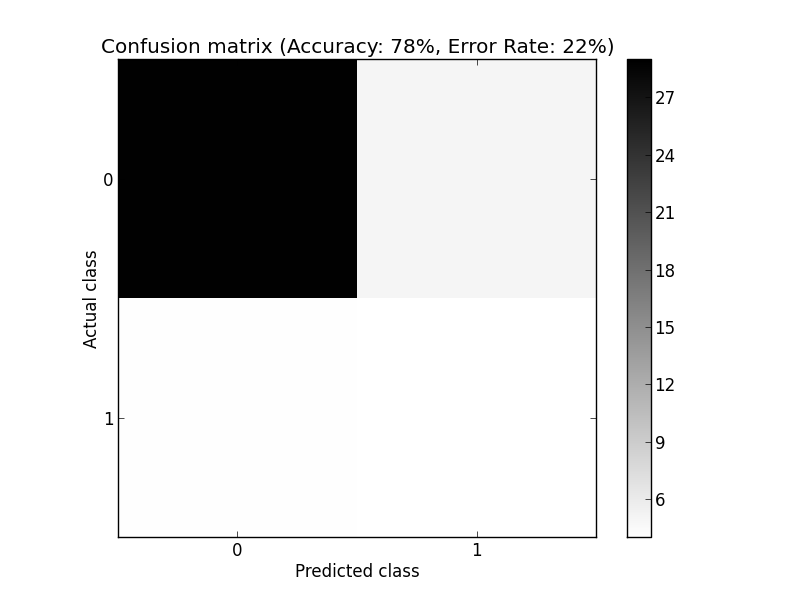
\includegraphics[scale=0.4]{pictures/cmX.png}
	\caption{Looking at all attributes.}
	\label{logicalRegressionResultX}
	\end{subfigure}
	\begin{subfigure}[b]{0.5\textwidth}
	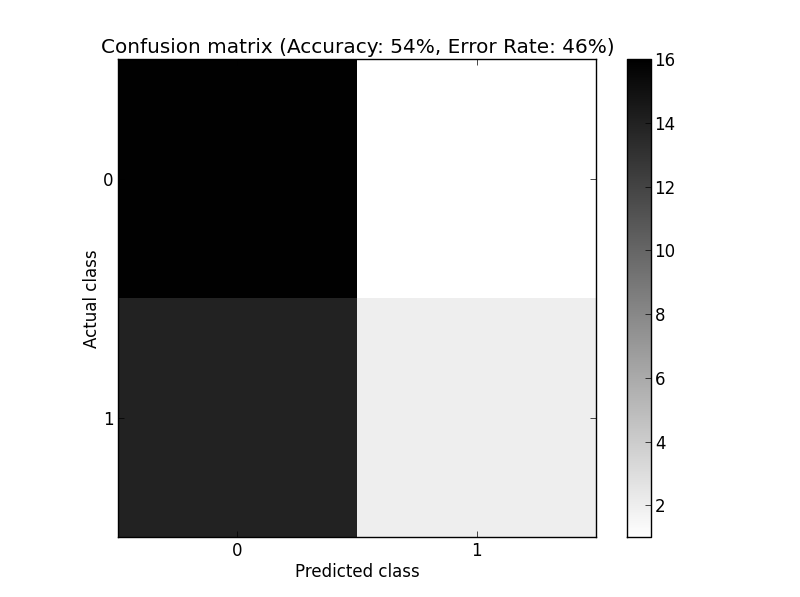
\includegraphics[scale=0.4]{pictures/cmXAD.png}	
	\caption{Looking at attributes selected by forward selection.}
	\label{logicalRegressionResultXad}
	\end{subfigure}

	\begin{subfigure}[b]{0.5\textwidth}
	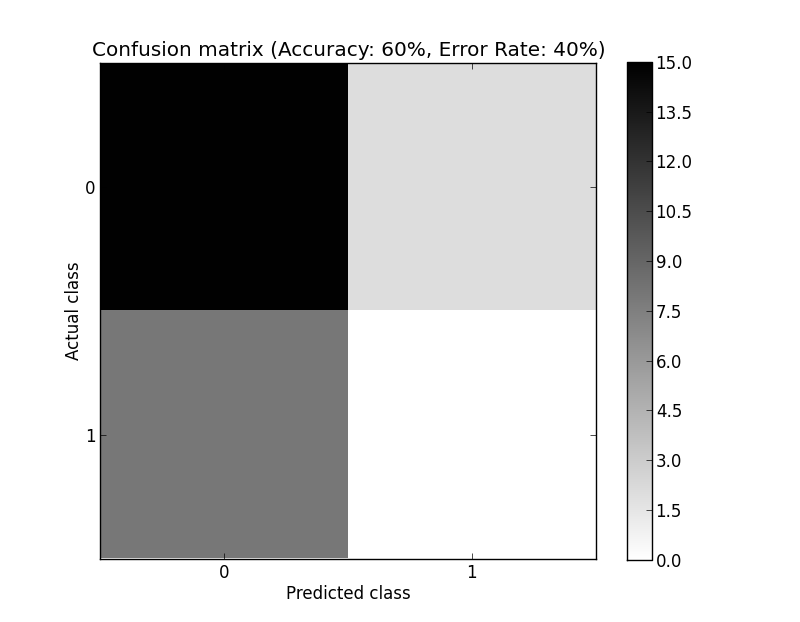
\includegraphics[scale=0.4]{pictures/cmPC.png}
	\caption{Looking at all principal components.}
	\label{logicalRegressionResultXPA}
	\end{subfigure}
	\begin{subfigure}[b]{0.5\textwidth}
	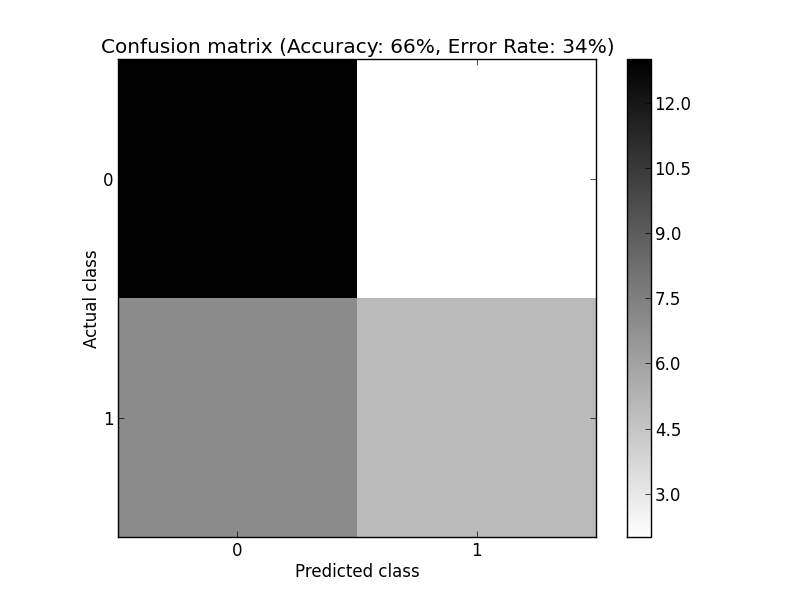
\includegraphics[scale=0.4]{pictures/cm2PC.png}
	\caption{Looking at two most important principal components.}
	\label{logicalRegressionResultX2PA}
	\end{subfigure}
\caption{This figure shows results of performing logical regression for different input.}
\label{logicalRegressionResults}
\end{figure}



We have compared the tree methods of classification with each other. For each method, we have looked at and calculated the misclassification rate, as described in sections (??TODO REF). However here we use the whole data set to describe the classification. And we then check the misclassification rate using the same data objects. Therefore we have also for these 3 approaches created random train and test sets. So we use a subset of our data set to train a classifier, and then we use another subset of the data set to estimate the misclassification. We have done this for 5 randomly generated sets. The results of this can be seen in \ref{misclasRes}. This figure indicates that Logical Regression (LR) is not very suitable for our data set. We also see that the misclassification results of Section (??TODO Ref) are quiet different from these. The table for instance shows us that Decision Trees might be better than eg. Logical Regression for our set.

\begin{table}
\begin{tabular}{|l|l|l|l|l|l|l|}
\hline
Method & test1 & test2 & test3 & test4 & test5 & Mean \\ \hline
LR / All attributes & 0.4792 & 0.2917 & 0.5 &   0.375 & 0.3333 & 0.3958\\ \hline
LR / According to FF & 0.3333 & 0.5208 & 0.4375 & 0.3125  &  0.3958 & 0.4    \\ \hline
LR / Principal Components & 0.4375  &  0.3333 & 0.4583 & 0.4167 & 0.3125 &     0.3917 \\ \hline
LR / Two most influence PC & 0.2917 & 0.3542 & 0.4167 & 0.3958 & 0.375    &   0.3667 \\ \hline

DT / All attributes & 0.3125  &    0.2917 & 0.4167 &  0.1875  &    0.25    &    0.2917 \\ \hline
DT / According to FF & 0.25    &    0.25 &    0.3958 & 0.3542 &  0.25    &    0.3        \\ \hline
DT / Principal Components & 0.2917 & 0.3958 & 0.3333 &  0.3542 &  0.2292 &  0.3208 \\ \hline
DT / Two most influence PC &  0.3333 & 0.3542 & 0.2917 & 0.3542 &  0.3542 &  0.3375  \\ \hline

KNN / All attributes & 0.3542 &  0.1458 & 0.5208 & 0.25 &    0.25 &       0.3042 \\ \hline
KNN / According to FF &  0.3333 &  0.3958 &  0.3958 &  0.4167 & 0.3125  &    0.3708 \\ \hline
KNN / Principal Components & 0.3333 &  0.3333 & 0.3333 &  0.3125   &   0.1875 &     0.3    \\ \hline
KNN / Two most influence PC & 0.2292 &  0.3333 &  0.3125  &  0.3333 &  0.3542 &  0.3125   \\ \hline

\end{tabular}
\caption{Calculating average misclassification for the methods.}
\label{misclasRes}
\end{table}

%In Figure \ref{misclasRes} we can see the results of c